% $Header: /cvsroot/latex-beamer/latex-beamer/solutions/conference-talks/conference-ornate-20min.de.tex,v 1.7 2004/10/07 20:53:08 tantau Exp $

\documentclass{beamer}

\mode<presentation>
{
  	\usetheme{Frankfurt}
  	\usecolortheme{seahorse}
	\useinnertheme{circles}  

  \setbeamercovered{transparent}
  % oder auch nicht
}

\usepackage{color}
\usepackage{graphicx}
\usepackage{epstopdf}


\usepackage[german]{babel}
% oder was auch immer

\usepackage[utf8]{inputenc}
% oder was auch immer

\usepackage{times}
\usepackage[T1]{fontenc}
% Oder was auch immer. Zu beachten ist, das Font und Encoding passen
% mssen. Falls T1 nicht funktioniert, kann man versuchen, die Zeile
% mit fontenc zu lschen.


\title[Pflichtenheft] % (optional, nur bei langen Titeln ntig)
{e-puck Conquest}

\subtitle
{Pflichtenheft}

\author[Autor, Anders] % (optional, nur bei vielen Autoren)
{SEP - ITS 2010 \\ Max Binder \and Florian Bürchner \and Martin Freund
	\\ Florian Lorenz \and Andreas Poxrucker \and Andreas Wilhelm}
% - Namen mssen in derselben Reihenfolge wie im Papier erscheinen.
% - Der \inst{?} Befehl sollte nur verwendet werden, wenn die Autoren
%   unterschiedlichen Instituten angehren.

\institute[Universität Passau] % (optional, aber oft ntig)
{
  Fakultät für Informatik und Mathematik\\
  Universität Passau}

\AtBeginSubsection[]
{
  \begin{frame}<beamer>
    \frametitle{Gliederung}
    \tableofcontents[currentsection,currentsubsection]
  \end{frame}
}


% Falls Aufzhlungen immer schrittweise gezeigt werden sollen, kann
% folgendes Kommando benutzt werden:

%\beamerdefaultoverlayspecification{<+->}



\begin{document}

\begin{frame}
  \titlepage
\end{frame}

\begin{frame}
  \frametitle{Gliederung}
  \tableofcontents
  % Die Option [pausesections] knnte ntzlich sein.
\end{frame}

\section{Einleitung}

\begin{frame}
  \frametitle{Motivation}
  \begin{figure}[htbp]
	\begin{minipage}[t]{5cm}
		\vspace{0pt}
		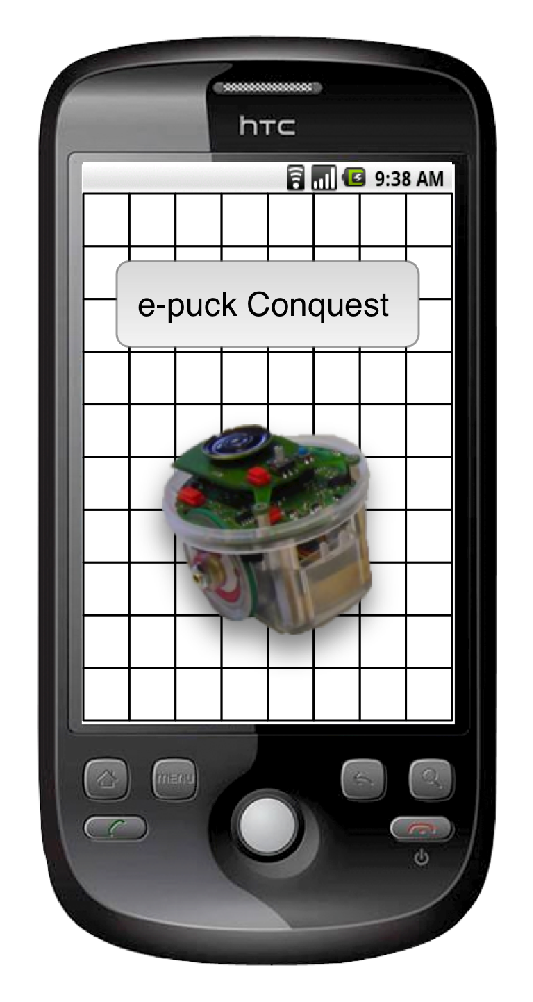
\includegraphics[height=5cm]{logo.eps} 
	\end{minipage}
	\hfill
	\begin{minipage}[t]{0.5\textwidth}
		\vspace{30pt}
		\begin{itemize}
			\item Einleitung
			\item Grobe Aufgabenstellung
			\item Vorstellung der Medien
		\end{itemize}
	\end{minipage}
   \end{figure}
\end{frame}

\begin{frame}
  \frametitle{Anwendungsbereiche}

Mögliche Anwendungen durch Erweiterungen unseres Systems sind:

	\begin{itemize}
	    \item Vermessung von Baugebieten
        \item Putzroboter für den Einsatz im Alltag
		\item Grundrisszeichnungen für Wohnungen
		\item Systematisches Absuchen von Gebieten
		\item Grundlagenforschung
	\end{itemize}

\end{frame}

\section{Aufgabenstellung}

\begin{frame}
  \frametitle{Kriterien aus dem Lastenheft}
  
	\begin{itemize}
		\item Erkundung von unbekannten Spielfeldern
		\item Kommunikation und Kooperation der e-puck Roboter ohne zentrale Steuereinheit 				(Master/Slave)
		\item Darstellung der bereits erkundeten Karte auf dem Smartphone sowie die 					aktuelle Position der Roboter
		\item Auswahl und Steuerung eines einzelnen e-puck Roboters
	\end{itemize}
	\vspace{15pt}
	\begin{center}
		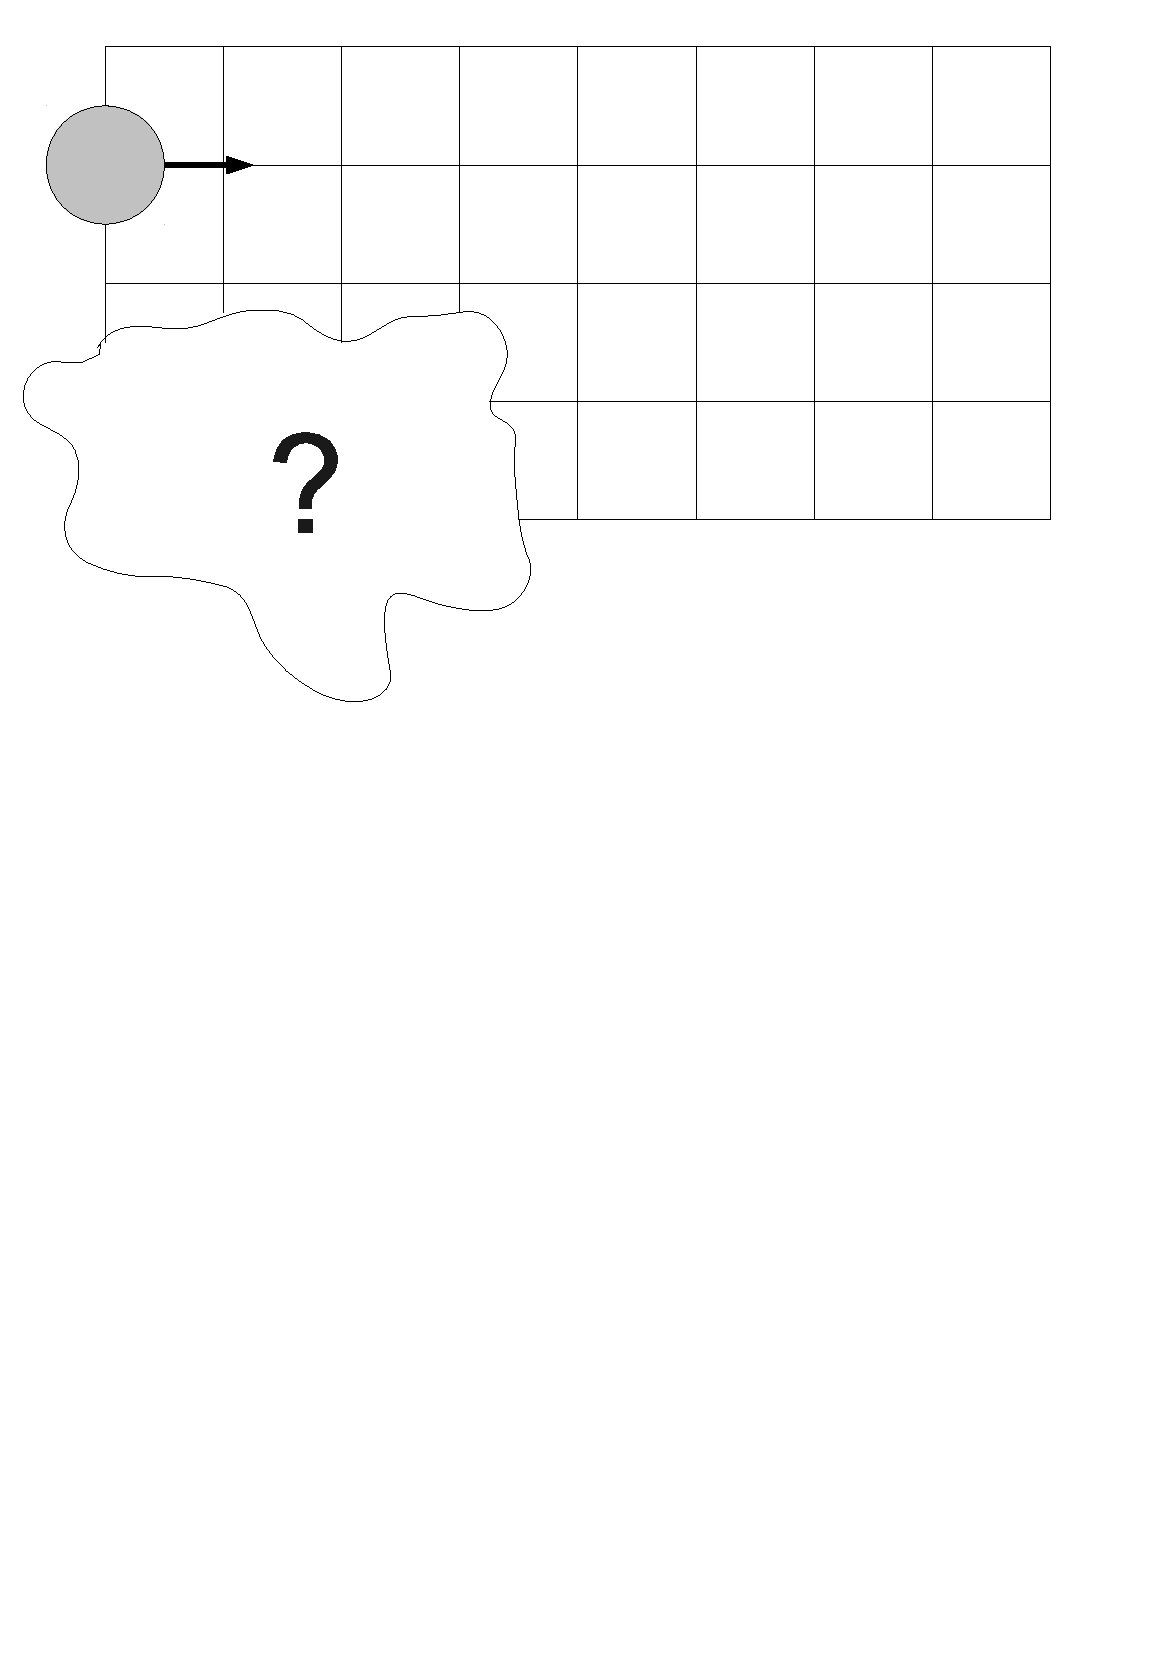
\includegraphics[width=6cm]{unerkundet.eps}  
	\end{center}
	
\end{frame}

\begin{frame}
  \frametitle{Kriterien aus dem Pflichtenheft}
  
  	\begin{itemize}
  		\item Linienverfolgung
		\item Genaue Rahmenbedingungen für das Spielfeld (Größe von Quadraten, usw.)
		\item Festdefinierte Startplätze
		\item Kollisionserkennung und Vermeidung
		\item Bluetoothkommunikation
		\item Steuerungsarten (On-Screen-Joystick, Kippsteuerung)
		\item Erkundete Felder
	\end{itemize}  
\end{frame}

\begin{frame}
  \frametitle{Wunschkriterien}
  	
	\begin{figure}[htbp]
	
	\begin{minipage}[t]{0.5\textwidth}
		\begin{itemize}
			\item Zustandsvisualisierung
			\item Beliebige Startpositionen
			\item Pfadanzeige von Robotern
			\item Exportfunktion für erkundete Karten
		\end{itemize}
	\end{minipage}
	\hfill
	\begin{minipage}[t]{5cm}
		\vspace{0pt}
		
\includegraphics[height=5cm]{idee.jpg} 
	\end{minipage}
   \end{figure}  	
\end{frame}


\section{Abgrenzungskriterien}

\begin{frame}
  \frametitle{Rahmenbedingungen}
		\begin{figure}[htbp]
			\begin{minipage}[]{7cm}
				\begin{itemize}
					\vspace{0pt}
					\item Keine ungültigen oder sich dynamisch ändernden Spielfelder
					\item Unterstützung von maximal einem Smartphone
					\item Größe des Spielfeldes
					\item Betriebsbedingungen
				\end{itemize} 
			\end{minipage}
			\begin{minipage}[t]{21cm}
				\vspace{30pt}
				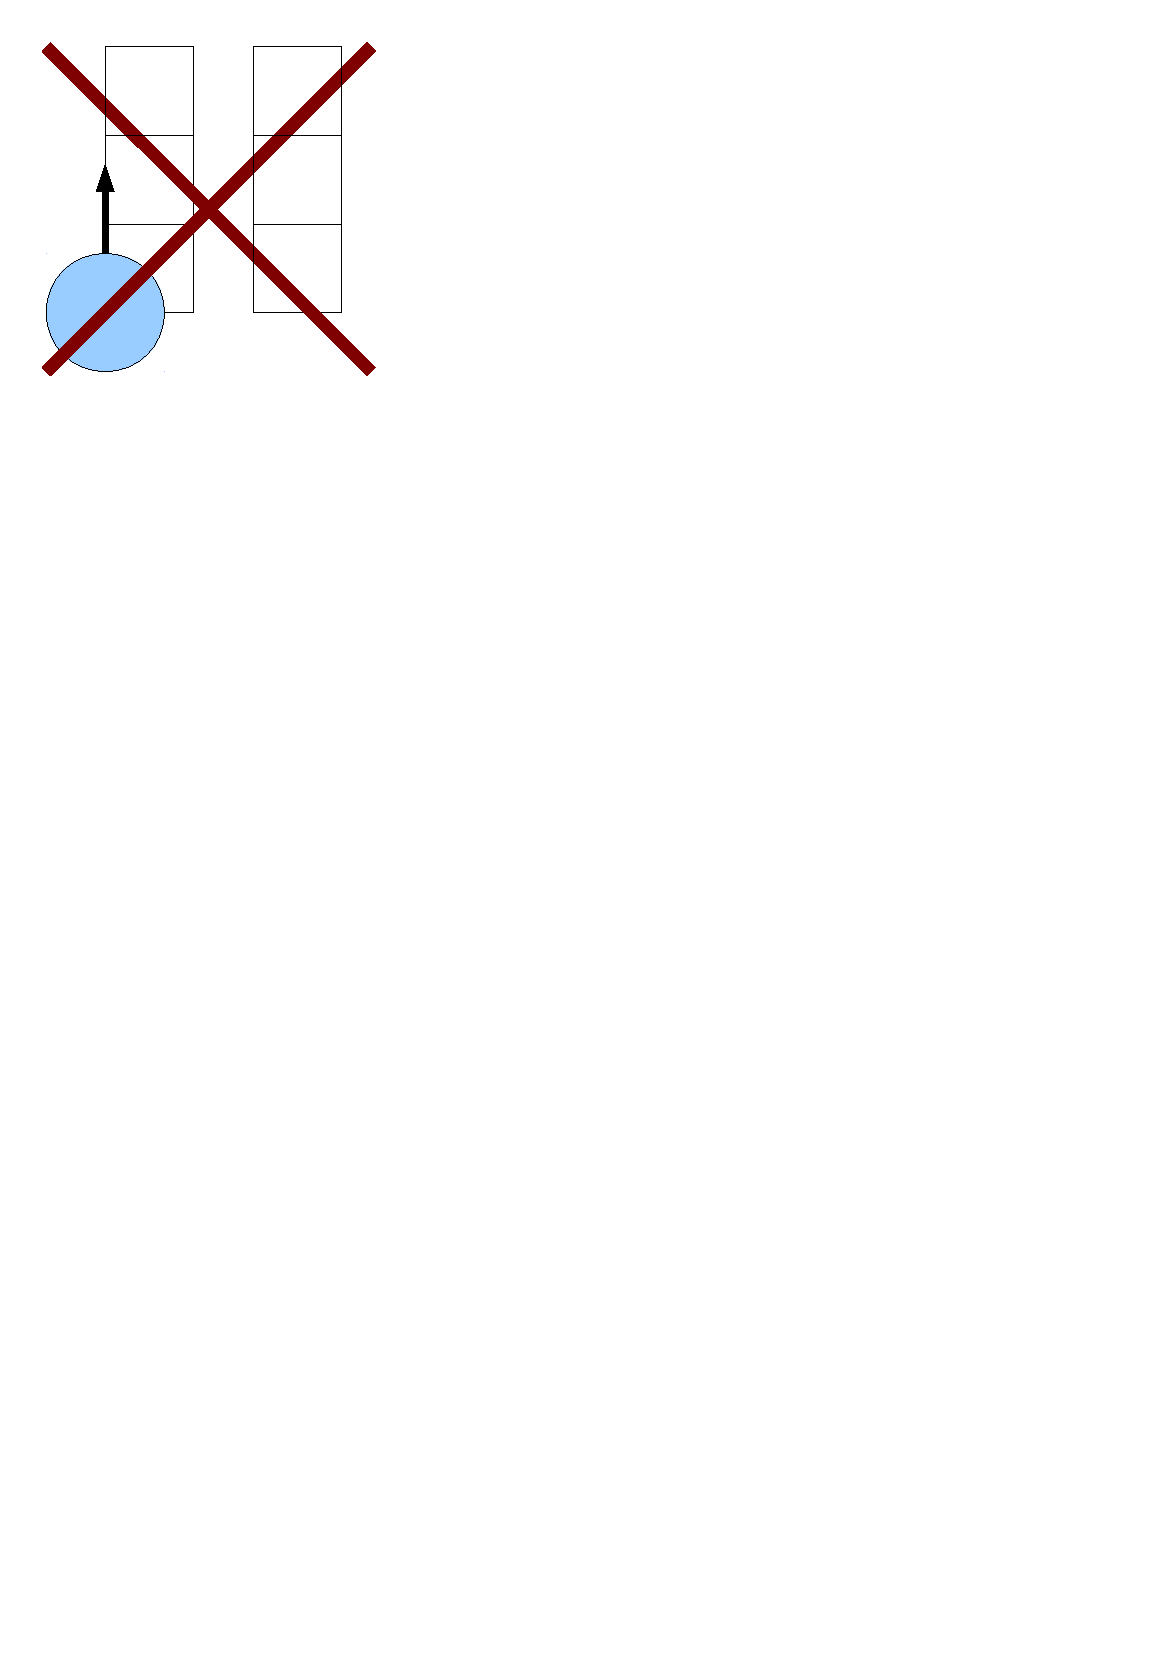
\includegraphics[height=7cm]{ungueltig1.eps}
				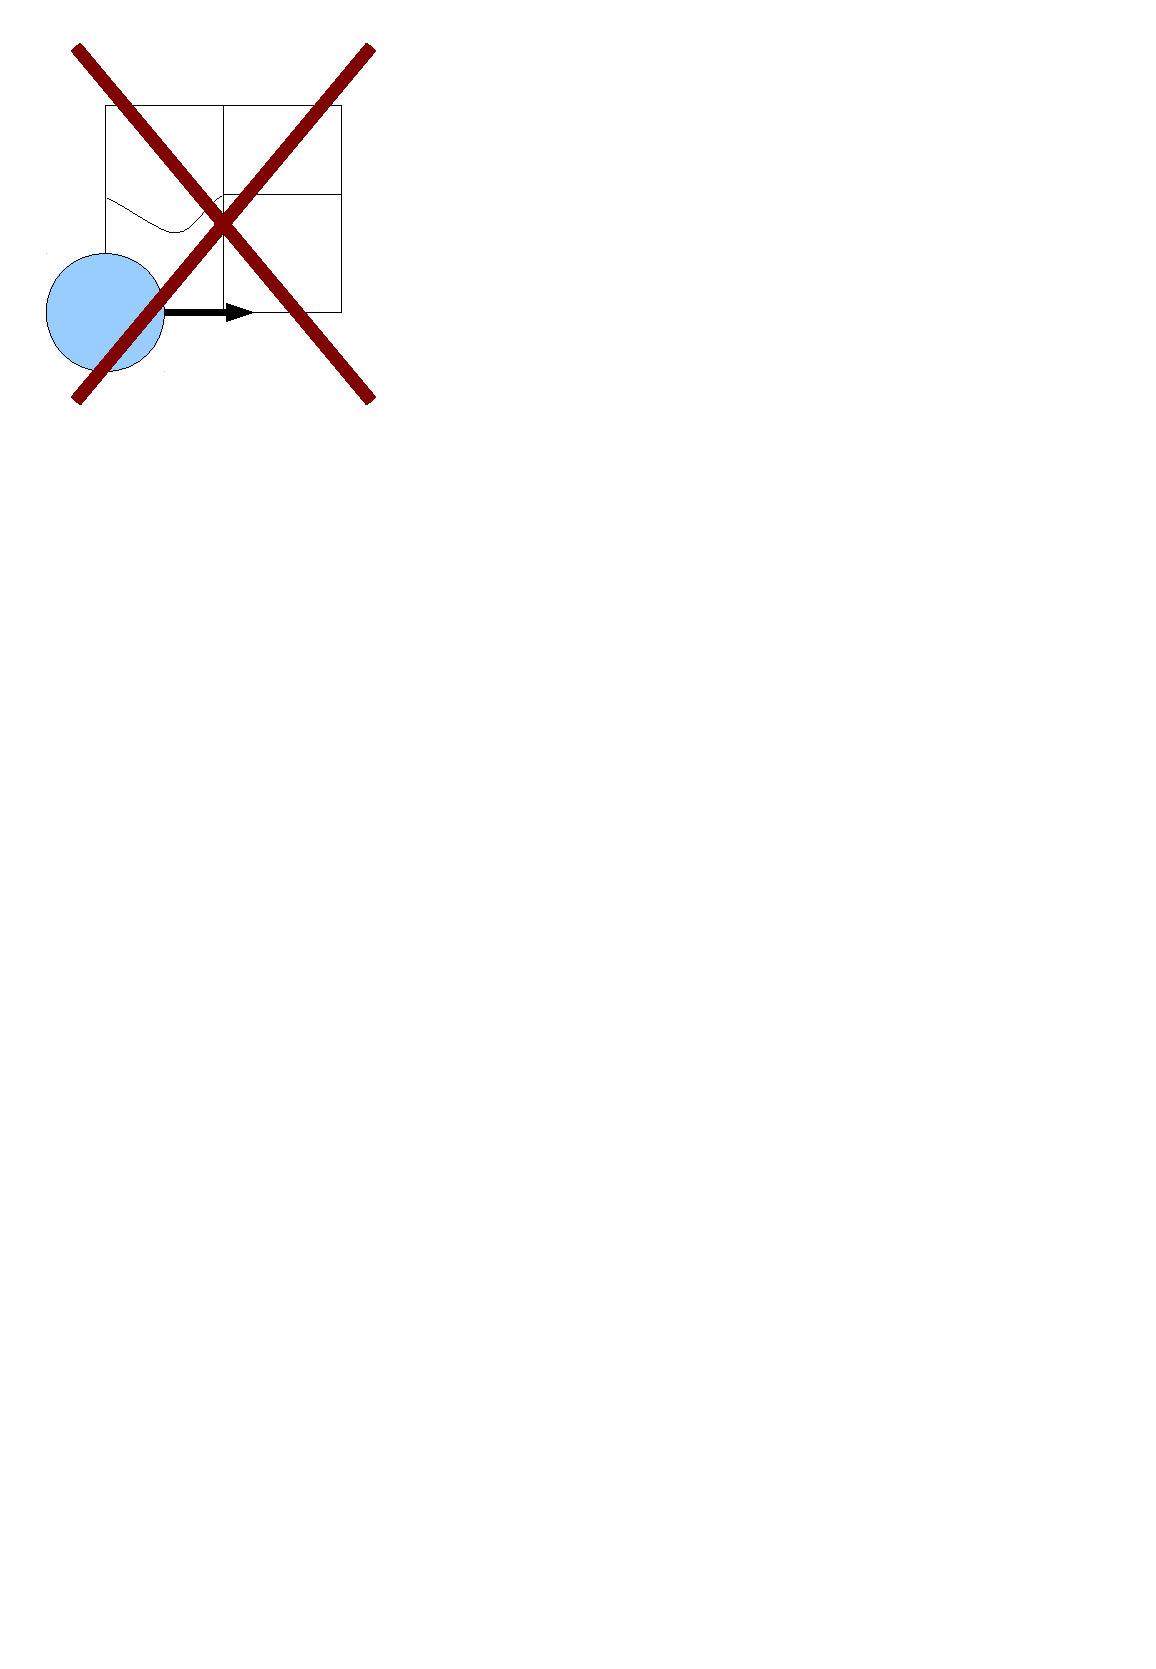
\includegraphics[height=7cm]{ungueltig2.eps} 
				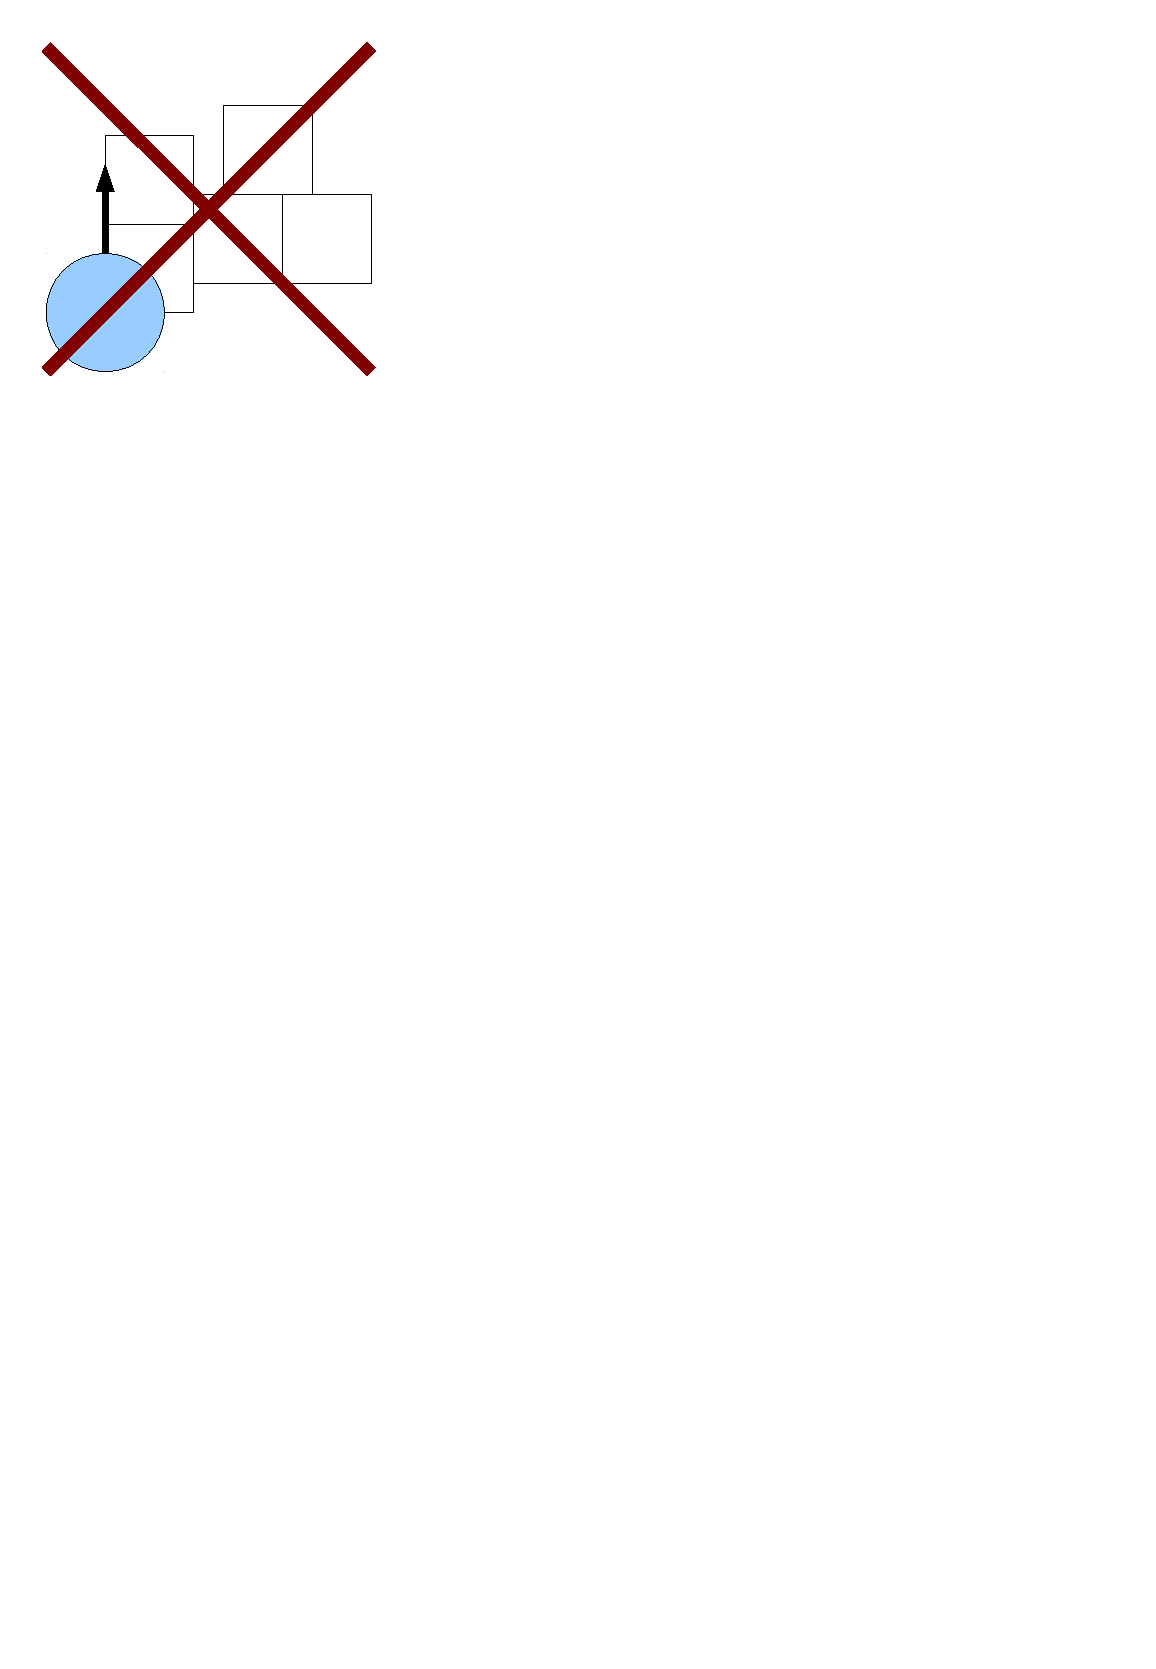
\includegraphics[height=7cm]{ungueltig3.eps} 
			\end{minipage}
   		\end{figure}
		
		
		 
\end{frame}

\section{Qualität}
\begin{frame}
  \frametitle{Qualitätsmerkmale}
	\begin{figure}[htbp]
	
	\begin{minipage}[t]{0.5\textwidth}
		\begin{itemize}
			\item Effizienz
			\item Korrektheit
			\item Wartbarkeit
			\item Erweiterbarkeit
			\item Robustheit
		\end{itemize}
	\end{minipage}
	\hfill
	\begin{minipage}[t]{5cm}
		\vspace{0pt}
		
\includegraphics[height=5cm]{qualitt.jpg} 
	\end{minipage}
   \end{figure}  	  
  
\end{frame}

\section{Funktionen}
\begin{frame}
  \frametitle{Funktionsgruppen}
  
  	\begin{itemize}
		\item Netzwerkfunktionen
		\item Bewegungsfunktionen
		\item Erkundungsfunktionen
		\item Handyfunktionen
		\item Allgmeine Funktionen
	\end{itemize}  
	\begin{figure}[bp]
		
\includegraphics[height=2cm]{funktional.jpg} 
	\end{figure}
	
\end{frame}

\section{Graphische Benutzeroberfläche}
\begin{frame}
  \frametitle{Funktionalitäten der Benutzeroberfläche}
  	\begin{itemize}
		\item Autoskalierung der Karte
		\item Auswahl der e-puck Roboter
		\item Kartendarstellung
		\item Auswahl der verschiedenen Steuerungsarten
		\item Statistik
	\end{itemize}  
	\vspace{1cm}
	\begin{figure}[bp]
		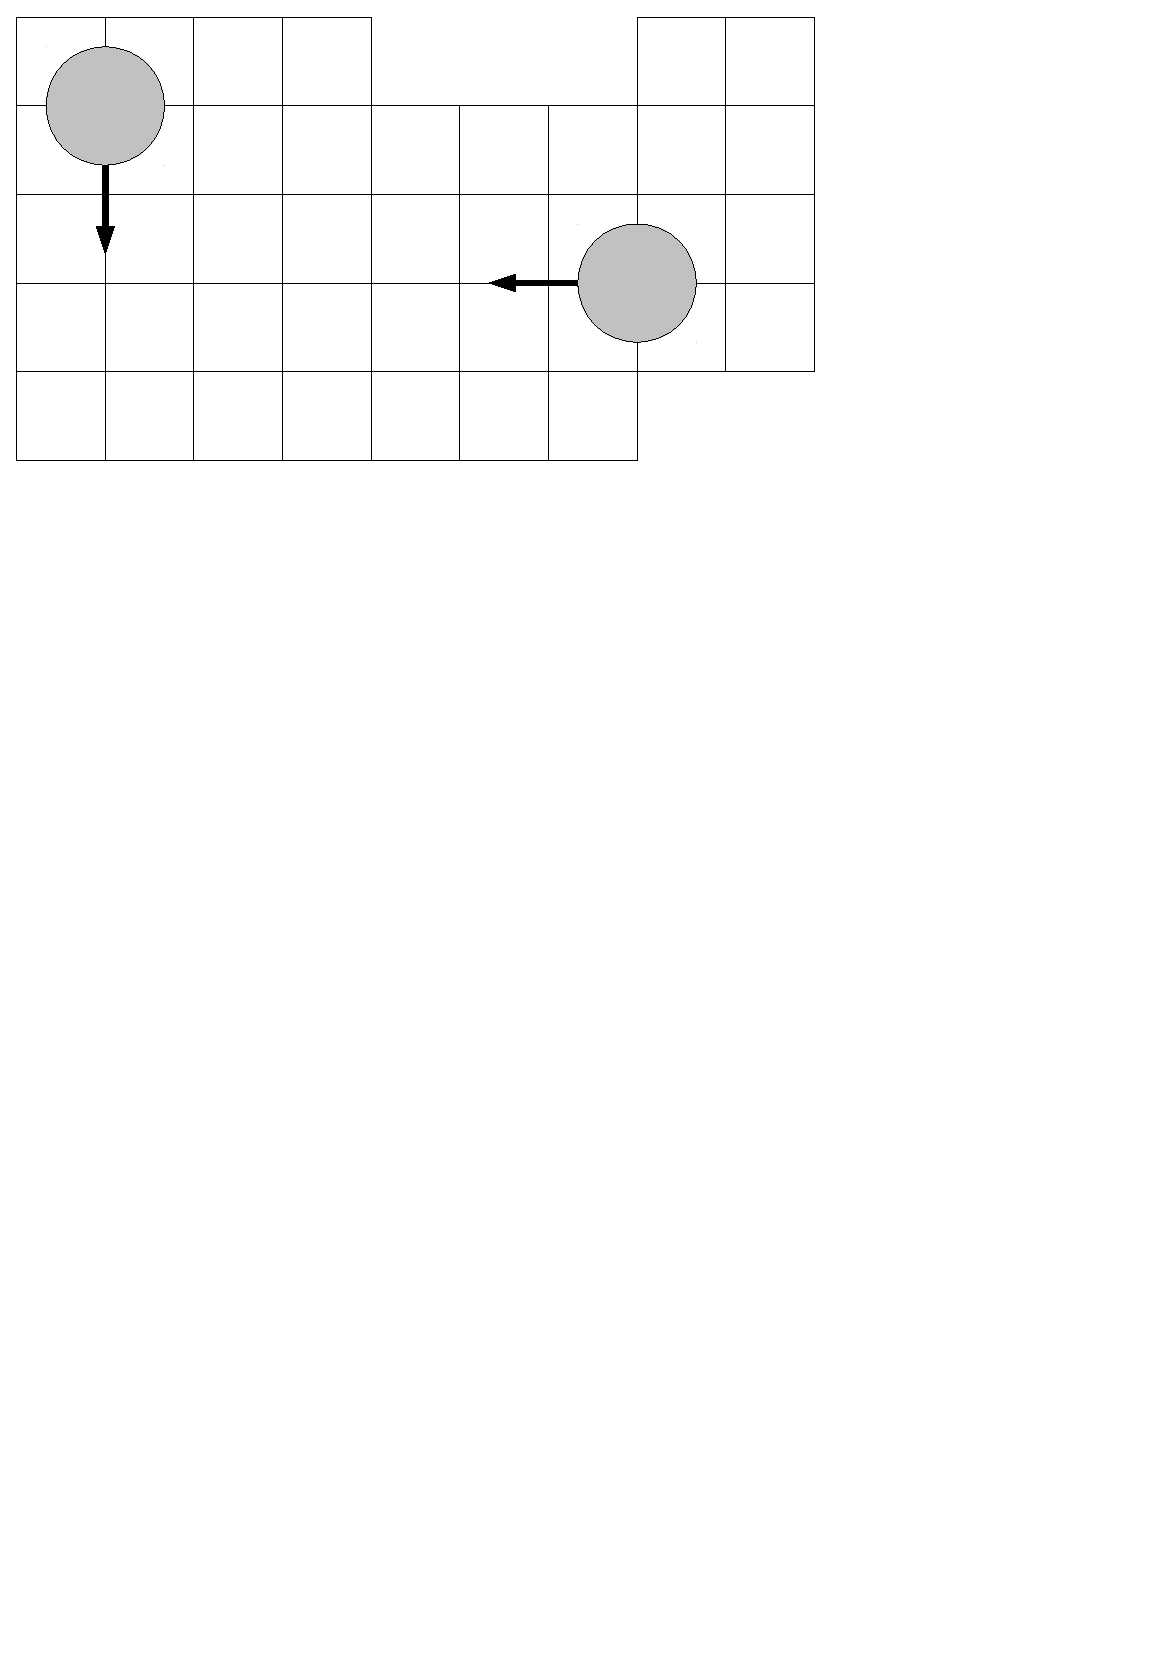
\includegraphics[height=12cm]{karte.eps} 
	\end{figure}
\end{frame}

\begin{frame}
  \frametitle{Beispieldialoge der Benutzeroberfläche}
	\begin{figure}[bp]
		\begin{minipage}[]{3.5cm}
			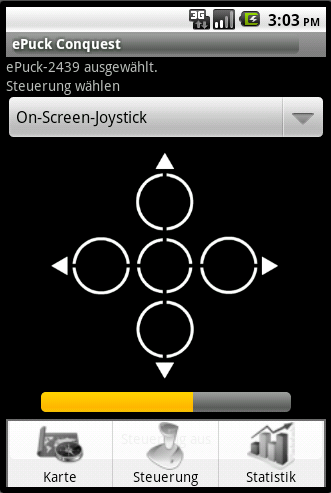
\includegraphics[height=5cm]{view1.png} 
			\caption{Steuerung}
		\end{minipage}
		\hspace{1cm}
		\begin{minipage}[]{3.5cm}
			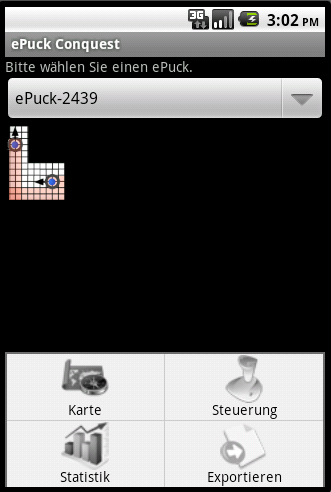
\includegraphics[height=5cm]{view2.png} 
			\caption{Karte}
		\end{minipage}
	\end{figure}
\end{frame}

\section{Tests}
\begin{frame}
  \frametitle{Testfälle}
  
  	\begin{itemize}
		\item Linien- und Knotenerkennung
		\item Broadcastsendetest
		\item Manuelle Steuerung mit Geschwindigkeitsänderung
		\item Export/Import Karte
		\item Erkundungstest mit und ohne globaler Lokalisierung
	\end{itemize}  
	
\end{frame}

\section{Fragen}
\begin{frame}
	\frametitle{Haben Sie noch Fragen?}
		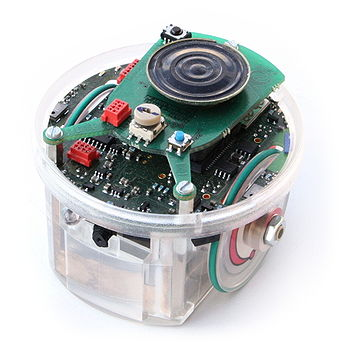
\includegraphics[height=4cm]{ende.jpg}
		\vspace{1cm}
	Vielen Dank für Ihre Aufmerksamkeit!
\end{frame}
\end{document}


